\documentclass[12pt,a4paper,portuguese]{article}
\usepackage[T1]{fontenc}
\usepackage{babel}
\usepackage{graphicx}
\usepackage{float}
\usepackage{pythonhighlight}

\title{Lista 6 - Análise de Séries Temporais em Oceanografia}
\author{Lucas Salimene}
\date{}
\begin{document}
\maketitle
\newpage

Utilizando as bibliotecas NumPy, Matplotlib, SciPy, Pandas e Pywt, foi desenvolvido a função:

\begin{python}
import numpy as np
import matplotlib.pyplot as plt
from scipy import signal
import pandas as pd
import pywt 
def wavelet(data,time,wavelet='morl',normal=True,filtro=True,alta=False):
if normal==True:
data_norm = (data - data.min())/ (data.max() - data.min())
data = data_norm
else:
data=data
data = pd.Series(data).interpolate().values
if filtro==True:
databaixa = signal.savgol_filter(data,73,2)
datasem = data
data = databaixa
else:
data=data
if alta==True:
data = datasem-databaixa
bfs, bPs = signal.welch(data)
cA, freq = pywt.cwt(data,np.arange(1, 2000), wavelet=wavelet)
power = (abs(cA))**2
period = 1./freq
plt.figure(figsize=(12,10))
plt.subplot(211)
plt.title('Welch')
plt.plot(bfs, bPs,'r')

f, ax = plt.subplots(figsize=(15, 10))
a=ax.contourf(time, np.log2(period), np.log2(power), 100,
extend='both')

ax.set_title(' Wavelet Power Spectrum ' )
ax.set_ylabel('Periodo')
ax.set_xlabel('Frequencia')

Yticks = 2 ** np.arange(np.ceil(np.log2(period.min())),
np.ceil(np.log2(period.max())))
ax.set_yticks(np.log2(Yticks))
ax.set_yticklabels(Yticks)
ax.invert_yaxis()
ylim = ax.get_ylim()
plt.colorbar(a)
plt.show()
\end{python}
Essa função irá realizar a transformada de Wavelet e a PSD pelo método de Welch a partir das variáveis \textcolor{blue}{data} e \textcolor{blue}{time}, ou seja uma variável $x$ e uma $t$. A função aceita os parâmetros \textcolor{red}{wavelet}, que define o tipo de transformada de Wavelet suportada pelo pacote Pywt se deseja realizar, sendo a padrão da do tipo morl. O parâmetro \textcolor{red}{normal} define se será realizada a normalização da série temporal. O parâmetro \textcolor{red}{filtro} define se será realizada a filtragem da série temporal e o parâmetro \textcolor{red}{alta} define se será realizada a filtragem para obter as altas frequências. 

O função pode ser utilizada da seguinte forma para o dado \textit{SST.mat}, que apresenta a temperatura da superfície do mar:
\begin{python}
wavelet(ssti,time)
\end{python}
Que irá retornar as figuras

\begin{figure}[H]
	\centering
	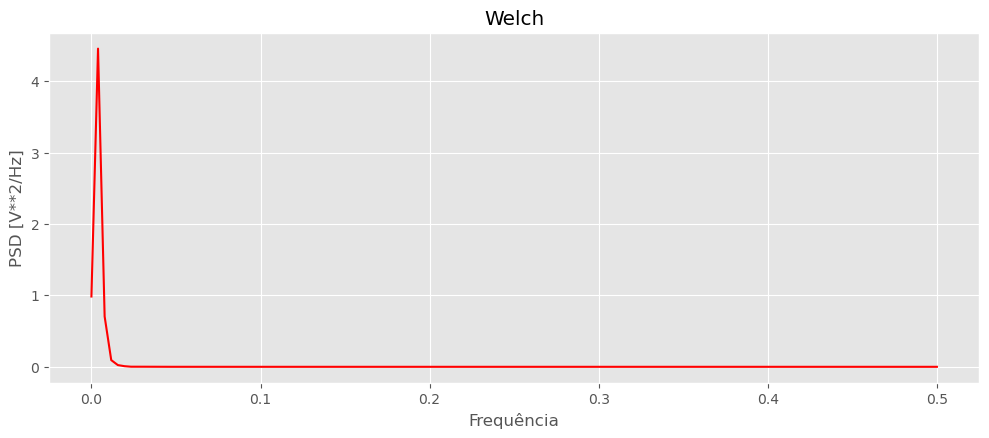
\includegraphics[width=1\linewidth]{lista6-1}
	\caption{PSD por Welch}
	\label{fig:lista6-1}
\end{figure}

\begin{figure}[H]
	\centering
	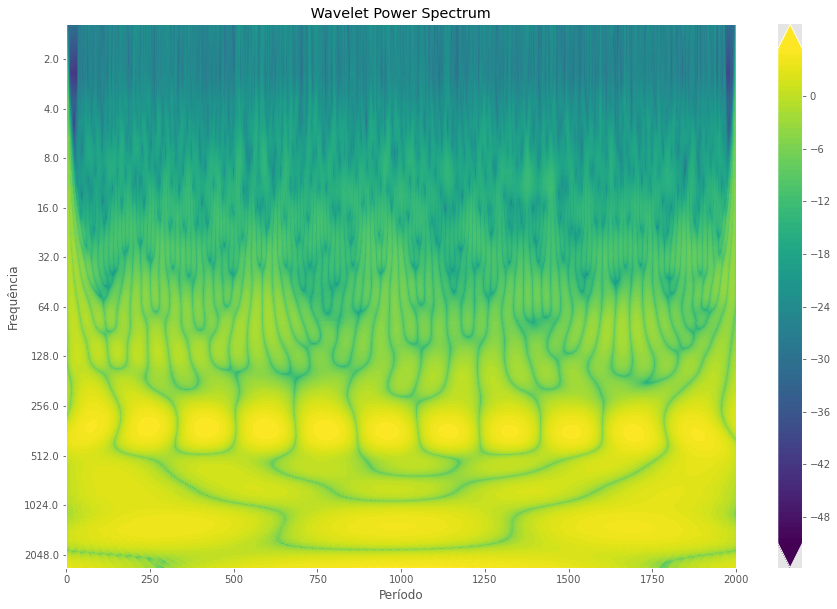
\includegraphics[width=1\linewidth]{lista6-2}
	\caption{Wavelet por morll}
	\label{fig:lista6-2}
\end{figure}

Caso se deseje mudar algum parâmetro, basta adicionar ele na chamada da função, por exemplo, para a wavelet do tipo chapéu mexicano se usaria:
\begin{python}
wavelet(ssti,time,wavelet='mexh')
\end{python}

\begin{figure}[H]
	\centering
	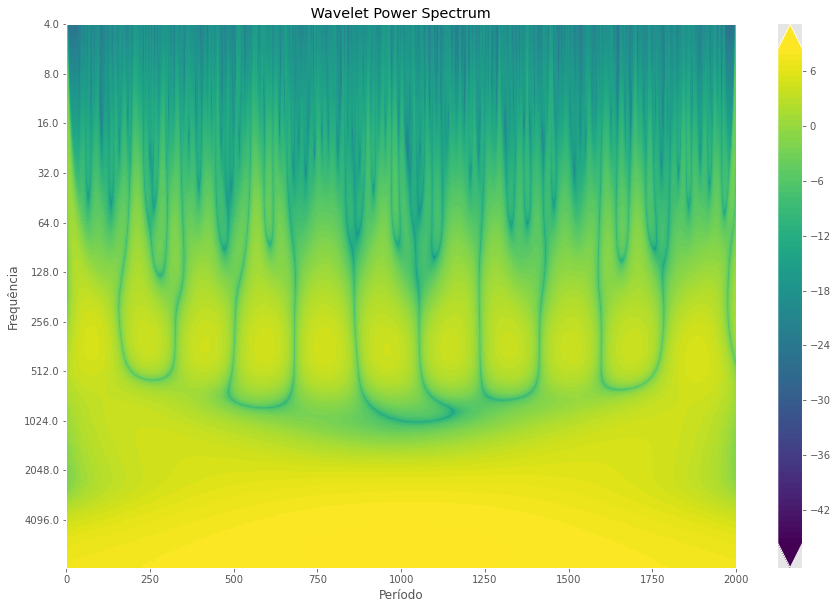
\includegraphics[width=1\linewidth]{lista6-3}
	\caption{Wavelet por mexh}
	\label{fig:lista6-3}
\end{figure}

Para uma wavelet do tipo de Gaus com a utilização de filtragem para apresentar as altas frequências:
\begin{python}
wavelet(ssti,time,alta=True,wavelet='gaus1')
\end{python}
\begin{figure}[H]
	\centering
	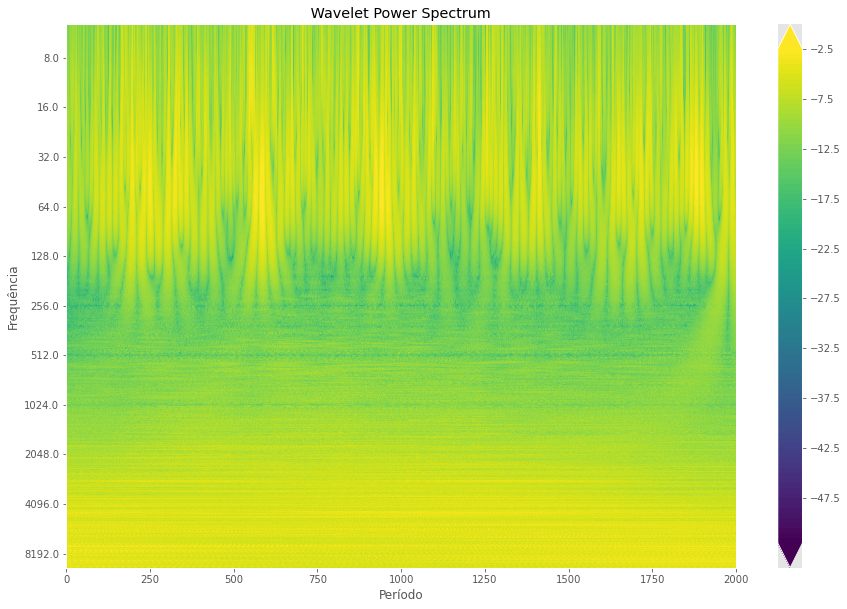
\includegraphics[width=1\linewidth]{lista6-4}
	\caption{Wavelet por gaus1 com filtragem nas altas frequências}
	\label{fig:lista6-4}
\end{figure}
Analisando a figura \ref{fig:lista6-2} se pode reparar a presença de de um sinal de alta frequência presente durante todo o período da serie temporal, e a presença de um sinal oscilante entre 64 Hz e 256Hz, com bastante ruído em frequência menores. \\

Ao utilizar a wavelet mãe do tipo chapéu mexicano, se obtém o resultado mostrado na figura \ref{fig:lista6-3}, onde o sinal de alta frequência sumiu e existe um sinal oscilante com picos a cada 250 períodos da série temporal.  \\

Utilizando um filtro para as altas frequências e uma wavelet mãe do tipo gaussiana, se obtém o resultado apresentado na figura \ref{fig:lista6-4}, onde todo o sinal de alta frequência foi retirado e sobra apenas os sinais oscilatórios na faixa de 64 Hz e 256 Hz, com um ruído melhor apresentado por esse método, permitindo a visualização de sinais de baixa frequência. \\

Outros resultados com wavelet mãe diferentes estão disponíveis no código do github.

\end{document}